\documentclass{standalone}
\usepackage{tikz}
\usetikzlibrary{arrows.meta}
\begin{document}
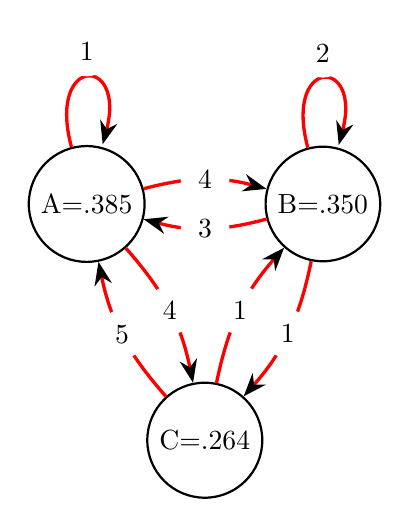
\begin{tikzpicture}
\begin{scope}[every node/.style={circle,thick,draw}]
    \node (A) at (0,3) {A=$.385$};
    \node (B) at (3,3) {B=$.350$};
    \node (C) at (1.5,0) {C=$.264$};
\end{scope}

\begin{scope}[>={Stealth[black]},
              every node/.style={fill=white,circle},
              every edge/.style={draw=red,very thick}]
		\path [->] (A) edge [loop above] node {$1$} (A);
    \path [->] (A) edge [bend left=15] node {$4$} (B);
    \path [->] (A) edge [bend left=15] node {$4$} (C);
		\path [->] (B) edge [bend left=15] node {$3$} (A);
    \path [->] (B) edge [loop above] node {$2$} (B);
    \path [->] (B) edge [bend left=15] node {$1$} (C);
		\path [->] (C) edge [bend left=15] node {$5$} (A);
    \path [->] (C) edge [bend left=15] node {$1$} (B);
\end{scope}
\end{tikzpicture}
\end{document}
